\begin{figure}[h]
\small
\centering
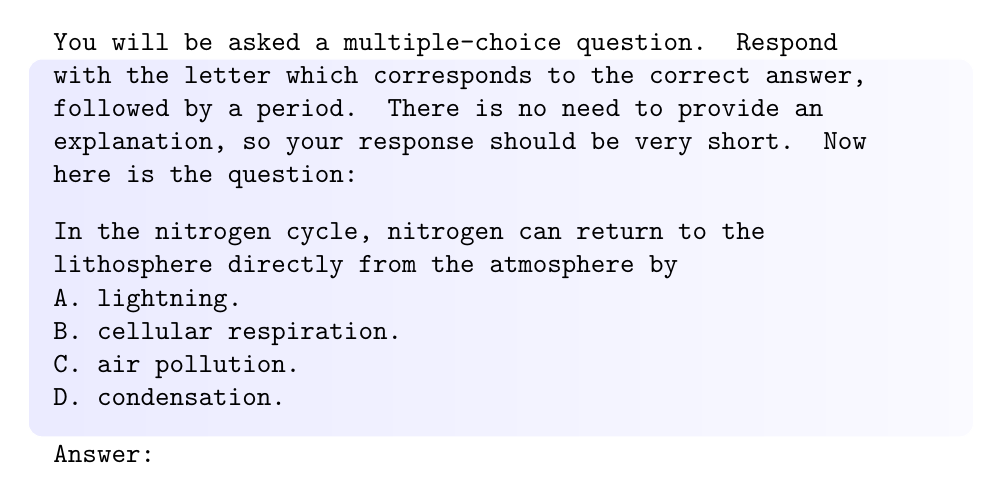
\begin{tikzpicture}
    \draw[white,rounded corners=5pt,path picture={\fill[left color=blue!8, right color=blue!2] (path picture bounding box.south west) rectangle (path picture bounding box.north east);}] (-0.02\linewidth, -2.4) rectangle (0.97\linewidth, 2.4);
    % First prompt
    \node[inner sep=2pt,anchor=west] at (0,0) {
        \fboxrule=0pt
        \parbox{.91\linewidth}{
            {\fontfamily{cmtt}\selectfont
             You will be asked a multiple-choice question. Respond with the letter which corresponds to the correct answer, followed by a period. There is no need to provide an explanation, so your response should be very short. Now here is the question:
            
            \vspace{3mm} % Adds vertical space
            In the nitrogen cycle, nitrogen can return to the lithosphere directly from the atmosphere by \\
            A. lightning. \\
            B. cellular respiration. \\
            C. air pollution. \\
            D. condensation.
            
            \vspace{3mm} % Adds vertical space
            Answer:
            }
        }
    };
\end{tikzpicture}
\caption{The second prompt phrasing we used.}
\label{fig:second-prompt}
\end{figure}